\section{Estimation de phase quantique (QPE)}
Soient une matrice unitaire quelconque $U$ et un de ses vecteurs propres $\ket*{\psi}$. Puisque la matrice est unitaire, on sait que la valeur propre associée à $\ket*{\psi}$ se situe sur le cercle du plan complexe, c'est-à-dire que $U\ket*{\psi} = e^{2\pi i \theta}\ket*{\psi}$ avec $\theta \in [0,1)$.  $U$ est une boîte noire qu'on peut utiliser mais dont on ne connaît rien, il n'est donc pas possible d'utiliser sa représentation matricielle pour trouver ses valeurs propres. L'estimation de phase quantique permet de donner une estimation de la valeur de $\theta$ (donc de la phase, d'où le nom) avec un certain degré de précision \cite{nielsen00}. En effet, on peut spécifier le nombre de qubits sur lesquels on stocke l'estimation de $\theta$. Donc, si $\theta$ s'écrit avec $t$ bits, alors une QPE avec un degré de précision à $m \ge t$ qubits donnera la réponse exacte. Au contraire, une QPE avec $m  < t$ qubits de précision donnera seulement une estimation à $m$ qubits de $\theta$.

Afin de réaliser la QPE, il faudra deux registres. Le premier registre contiendra $m$ qubits tous à $\ket*{0}$. C'est sur ces qubits qu'on stockera l'approximation de $\theta$. Le deuxième registre contient lui le vecteur propre $\ket*{\psi}$ dont on cherche la valeur propre. Donc, on suppose qu'on est capable de préparer $\ket*{\psi}$ au préalable de manière efficace. La première étape de la QPE consiste à appliquer une porte Hadamard sur chacun des qubits du premier registre afin de créer une superposition uniforme. Puis, on applique une série de portes $U^{2^k}$ pour $k \in [0, ..., m-1 ]$ chacune contrôlée par un qubit différent du premier registre. Son action permet d'ajouter une phase relative $e^{2\pi i 2^k \theta}$.

\begin{equation*}
    CU{2^k}\left(\frac{1}{\sqrt{2}}\left(\ket*{0\psi} + \ket*{1\psi}\right)\right) = \frac{1}{\sqrt{2}}\left(\ket*{0} + e^{2\pi i 2^k \theta}\ket*{1}\right) \ket*{\psi}
\end{equation*}

Comme $\theta$ est compris dans l'intervalle $[0,1)$ et qu'on a $m$ qubits de stockage, on peut utiliser la représentation binaire décimale pour dire que $\theta = 0\pmb{.}\theta_{m-1}...\theta_{0} = 0 + \theta_{m-1}2^{-1} + ... + \theta_{0}2^{-m}$. Ainsi, $2^k \theta$ décale les bits constituant $\theta$ de $k$ positions vers la gauche. Par exemple, 

\begin{equation*}
    2^0 \theta = 0\pmb{.}\theta_{m-1}...\theta_0, \ 2^1 \theta = \theta_{m-1}\pmb{.}\theta_{m-2}...\theta_0, \ ..., \ 2^{m-1}\theta = \theta_{m-1}...\theta_1\pmb{.}\theta_0
\end{equation*}

La partie entière de $2^k\theta$, comme on le sait, n'a aucun impact sur l'exponentielle $e^{2\pi i 2^k\theta}$. De ce fait, on ne garde que la partie fractionnaire. 

\begin{equation*}
    \frac{1}{\sqrt{2}}\left(\ket*{0} + e^{2\pi i 2^k \theta}\ket*{1}\right) \ket*{\psi} = \frac{1}{\sqrt{2}}\left(\ket*{0} + e^{2\pi i \ 0\pmb{.}\theta_{m-1-k}...\theta_0}\ket*{1}\right) \ket*{\psi}  
\end{equation*} 

Si on applique une porte $CU^{2^0}$ contrôlée par le dernier qubit du premier registre, une porte $CU^{2^1}$ contrôlée par l'avant-dernier qubit du premier registre et ainsi de suite jusqu'à une porte $CU^{2^{m-1}}$ contrôlée par le premier qubit du premier registre, alors on se retrouve avec un état particulier sur le premier registre.

\begin{equation*}
    \left[\frac{1}{\sqrt{2^m}} \bigotimes_{k=0}^{m-1} \left(\ket*{0} + e^{2\pi i \ 0\pmb{.}\theta_{k}...\theta_0}\ket*{1}\right)\right]\ket*{\psi} = \frac{1}{\sqrt{2^m}} \left[\left(\ket*{0} + e^{2\pi i \ 0\pmb{.}\theta_{m-1}...\theta_0} \ket*{1}\right) \otimes ... \otimes \left(\ket*{0} + e^{2\pi i \ 0\pmb{.}\theta_0 } \ket*{1}\right) \right] \ket*{\psi}
\end{equation*}

Il s'agit de l'état $\ket*{\theta}$ auquel on aurait appliqué la QFT. Comme la valeur de $\theta$ se trouve dans cet état, on applique ensuite la QFT inverse pour l'obtenir. Finalement, on mesure les qubits du premier registre afin d'avoir le résultat de l'approximation de $\theta$, ce qui permet d'approximer la valeur propre du vecteur propre $\ket*{\psi}$ de $U$. Puisque $\theta$ est une valeur décimale par définition, il faut faire attention à convertir sa valeur binaire en sa valeur numérique selon la représentation binaire décimale. Comme le vecteur propre dans le second registre reste inchangé, on peut relancer la QPE plusieurs fois en choisissant comme phase le résultat le plus fréquent dans le but d'avoir une meilleure approximation.

\begin{figure}[H]
    \centering
    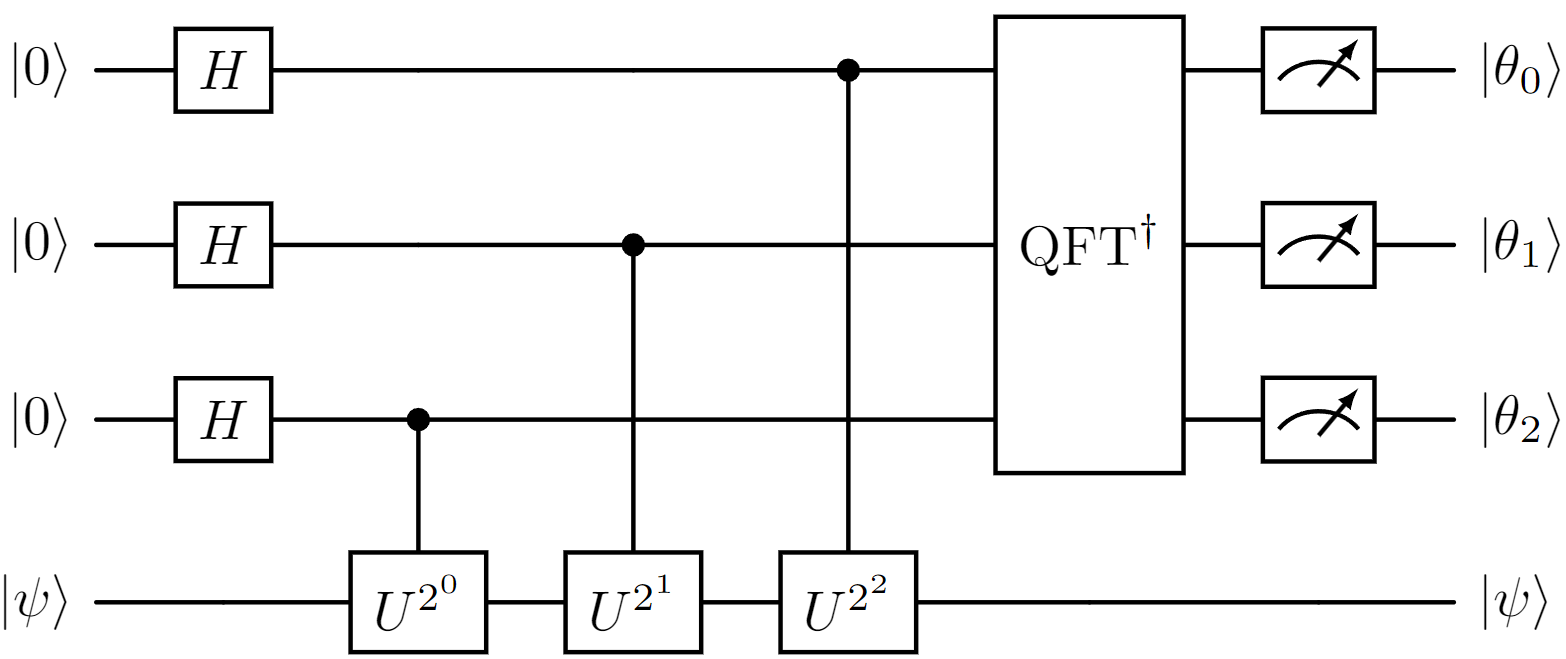
\includegraphics[scale=0.3]{images/circuit_qpe.png}
    \caption{Circuit de la QPE pour $m=3$}
\end{figure}

Pour utiliser moins de qubits dans le premier registre, on peut se servir du \textit{one qubit trick} \cite{Parker_2000}. Au lieu d'avoir $m$ qubits qui stockent l'approximation ou la valeur exacte de $\theta$, on peut en prendre un seul afin de connaître bit par bit la valeur de la phase. On commence par développer le circuit de la QFT$^\dag$ à la figure 2. 

\begin{figure}[H]
    \centering
    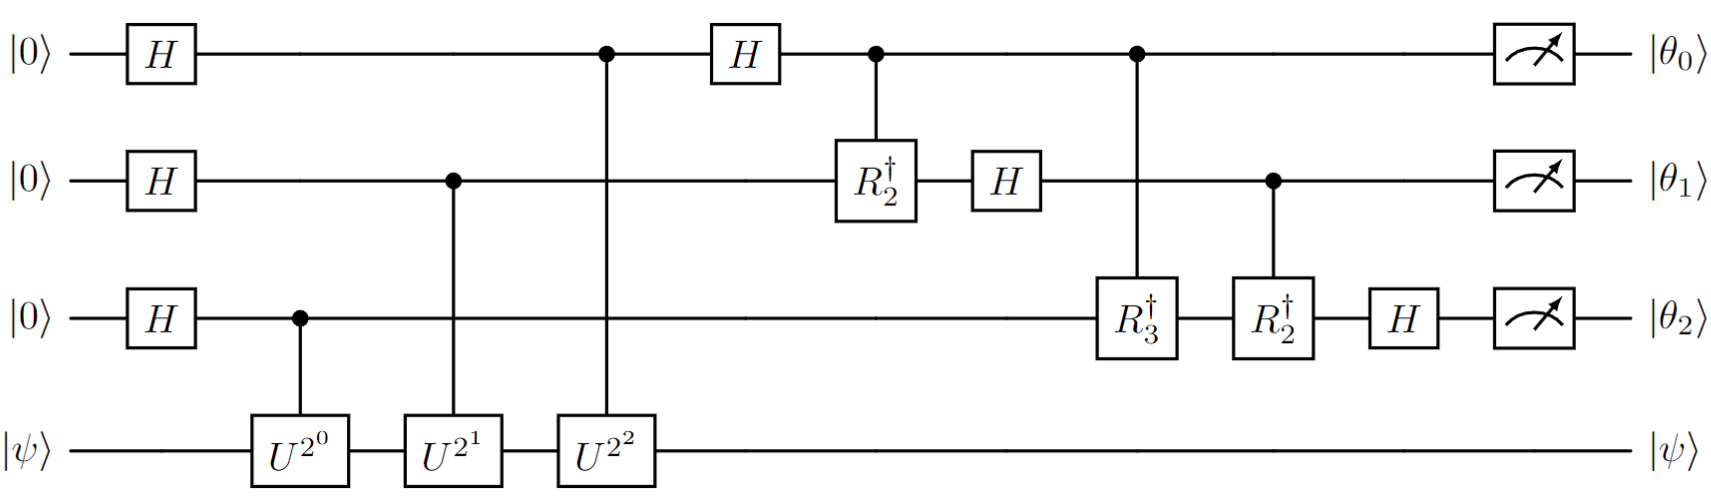
\includegraphics[scale=0.37]{images/qpe_etendue.png}
    \caption{Développement du circuit de la QPE pour $m = 3$}
\end{figure}

On s'attarde ensuite au premier qubit (celui tout en haut de la figure 3). Après la deuxième porte Hadamard, ce qubit sert de qubit de contrôle pour des portes de phase qui ne l'affectent aucunement. Puis, on mesure ce qubit. Si l'état après la mesure est $\ket*{0}$, puisque les portes contrôlées de phase ne changent pas ce qubit, cela veut dire que le qubit était aussi dans l'état $\ket*{0}$ avant leur application sur les autres qubits. La même logique s'applique si on avait eu l'état $\ket*{1}$.  De ce fait, on pourrait mesurer le premier qubit avant les portes de phase puis les ajouter après coup au circuit selon la mesure. De surcroît, en poussant plus loin la précédente réflexion, on voit que toutes les opérations sur le premier qubit (du tout début du circuit jusqu'à la mesure) peuvent être effectuées avant même celles des autres qubits. En fait, si on applique cette logique sur tout le premier registre, on voit qu'il est possible d'effectuer les opérations de chaque qubit successivement en appliquant manuellement les portes de phase selon la valeur des mesures passées. Grâce à cela, on peut utiliser un seul qubit afin de faire ce qu'on ferait normalement avec $m$ qubits sur  le premier registre. C'est ce qu'on appelle le \textit{one qubit trick} et il permet, au détriment de la profondeur, de réduire le nombre de qubits requis pour estimer la phase. 

\begin{figure}[H]
    \centering
    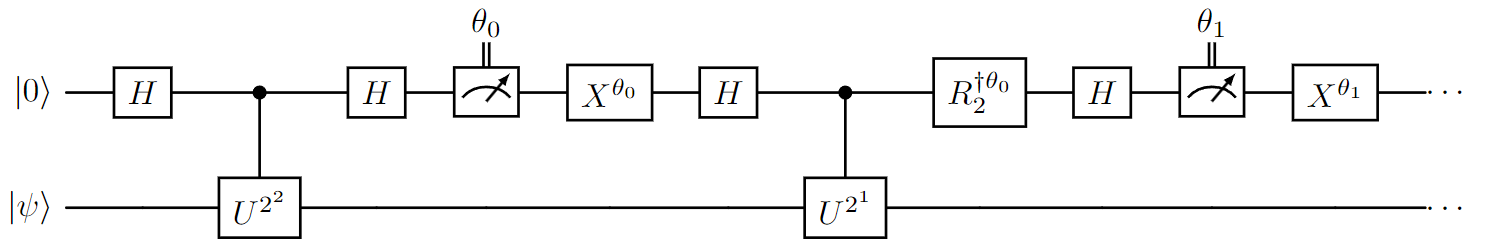
\includegraphics[scale=0.44]{images/one_qubit_trick.png}
    \caption{Le \textit{one qubit trick} pour une partie du circuit de la figure 3}
\end{figure}